\documentclass[12pt]{report}
\usepackage[utf8]{inputenc}
\usepackage[a4paper, margin=1in]{geometry}
\usepackage{graphicx}
\usepackage{lmodern}
\usepackage{setspace}
\usepackage{titling}
\usepackage{natbib}
\usepackage{url} % Add this line to handle URLs in bibliography
\usepackage{tabularx} % Ensure this package is loaded for extended table functionality

\begin{document}
\begin{titlepage}
    \centering
    \vspace*{1cm}
    {\Huge\bfseries What are the main theoretical barriers to resolving P vs NP?\par}
    \vspace{1cm}
    {\Large\itshape An Extended Project Qualification Dissertation\/\par}
    \vspace{1cm}
    {\Large Camron Short\par}
    {\large Candidate Number: 6439\par}
    {\large Centre Number: 19216\par}
    {\small GitHub Link: https://github.com/Skixrr/EPQ\par}
    \vspace{0.7cm}
    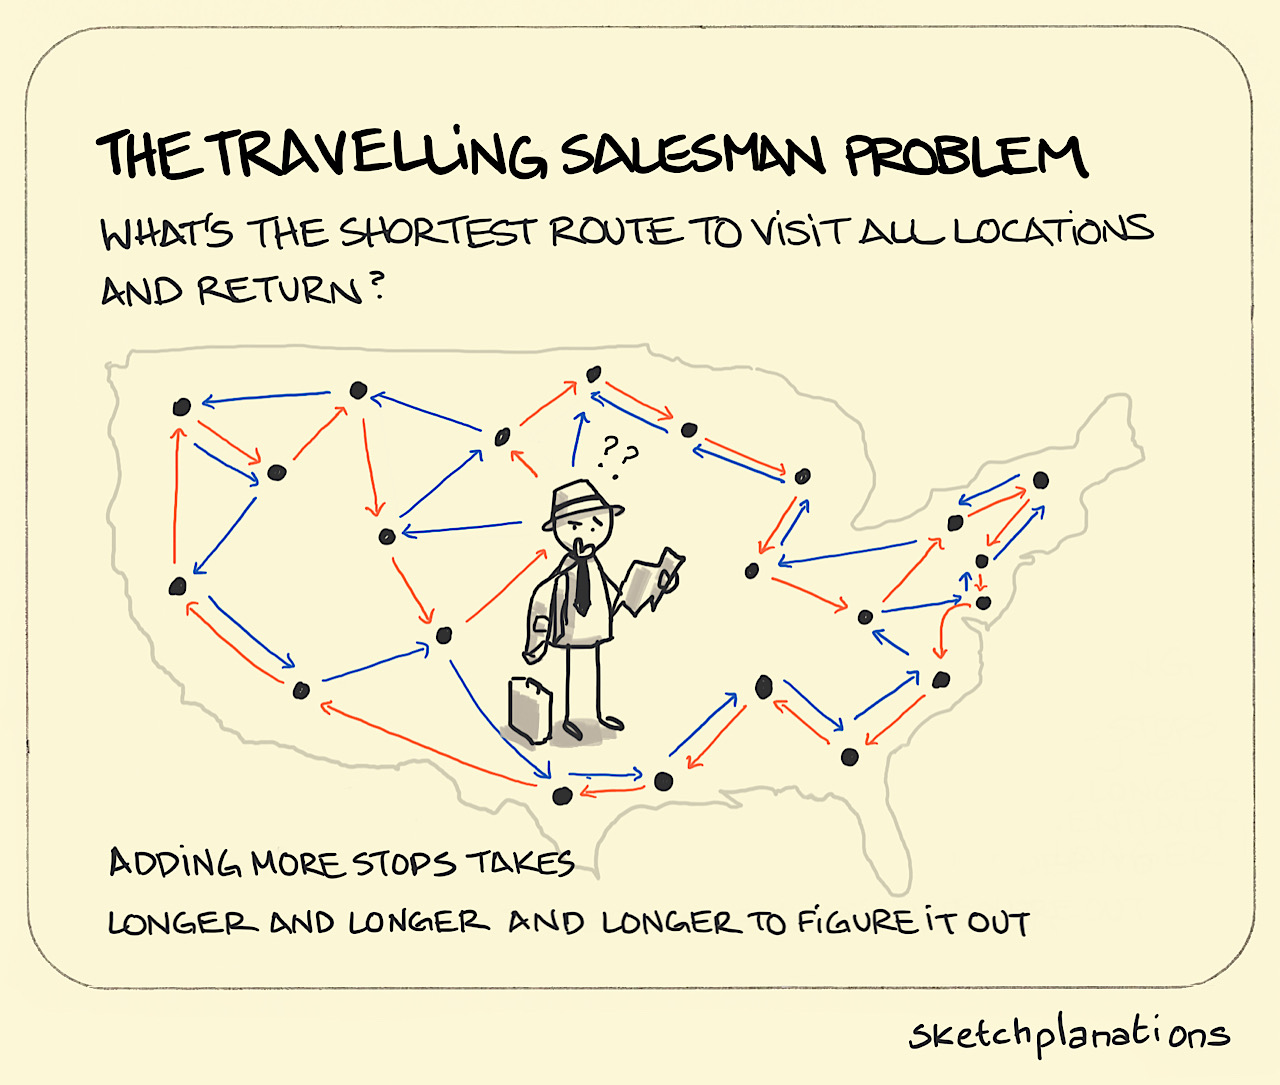
\includegraphics[width=1\textwidth]{CoverPhoto.jpg}
    \thispagestyle{empty}
\end{titlepage}

\section*{Timeline of Milestones}
\begin{center}
\begin{tabularx}{\textwidth}{|c|X|}
\hline
\textbf{Year} & \textbf{Milestone} \\
\hline
1956 & Gödel proposes the core question~\cite{godel1956} \\
\hline
1971 & Cook formalises P vs NP~\cite{cook1971} \\
\hline
1972 & Karp expands NP-completeness~\cite{karp1972} \\
\hline
1975 & Relativisation barrier identified~\cite{baker1975} \\
\hline
1994 & Natural proofs barrier defined~\cite{razborov1994} \\
\hline
2000 & Millennium Prize announced~\cite{claymillennium} \\
\hline
2008 & Algebrisation barrier introduced~\cite{arora2009, aaronson2008algebrization} \\
\hline
\end{tabularx}
\end{center}

\section*{A problem that resists solution}
The central question is \textbf{P vs NP}, one of the most famous problems in mathematics and computer science:
\begin{quote}
If we can verify a solution quickly, can we also find that solution quickly?
\end{quote}
This problem emerged naturally through the foundational research into logic and computation, only recieving Formalisation in the 1970s.
\vspace{0.4cm}
\paragraph{1956\,--\,Gödel's Insight}
Famous and renowned mathematician \textit{Kurt Gödel} wrote to another called Von Neumann, speculating whether checking a solution was significantly easier than discovering one.
Although unpublished, this idea became the basis of our current $\mathbf{P}$ vs $\mathbf{NP}$ problem~\cite{godel1956}.

\paragraph{1971\,--\,Cook's Formalisation}
\textit{Stephen Cook}, another mathematician, defined the problem formally in his paper~\cite{cook1971}.
He introduced our "complexity classes" --- we will go into what these are later as well as what they mean --- $\mathbf{P}$ and $\mathbf{NP}$.

\paragraph{1972\,--\,Karp's Expansion}
\textit{Richard Karp} built upon the work by Cook by demonstrating that many common problems relying on groupings or arrangements of objects are $\mathbf{NP}$~\cite{karp1972}.
This showed the problem's relevance to a vast amount of people.

\paragraph{2000\,--\,A Millennium Prize}
The \textit{Clay Mathematics Institute}, upon recognising the importance of \textbf{$\mathbf{P}$ vs $\mathbf{NP}$}, included it as one of their seven "Millennium Prize Problems", offering \$1,000,000 for anyone who could provide a correct proof~\cite{claymillennium}.

\section*{What are we doing?}
Within this paper I intend to explain why the greatest minds have yet to solve a major problem within mathmatics.


\newpage
\chapter{Defining the Problem}
\section{Introduction to our case study}
This report uses the travelling salesperson problem (TSP), a classic NP-complete problem, to illustrate key concepts in computational complexity. The objective is to find the shortest route visiting each location exactly once and returning to the start.%
\footnote{The salesperson metaphor is used for clarity: imagine planning a route that minimises travel distance or time.}
A simple example is shown below:\\
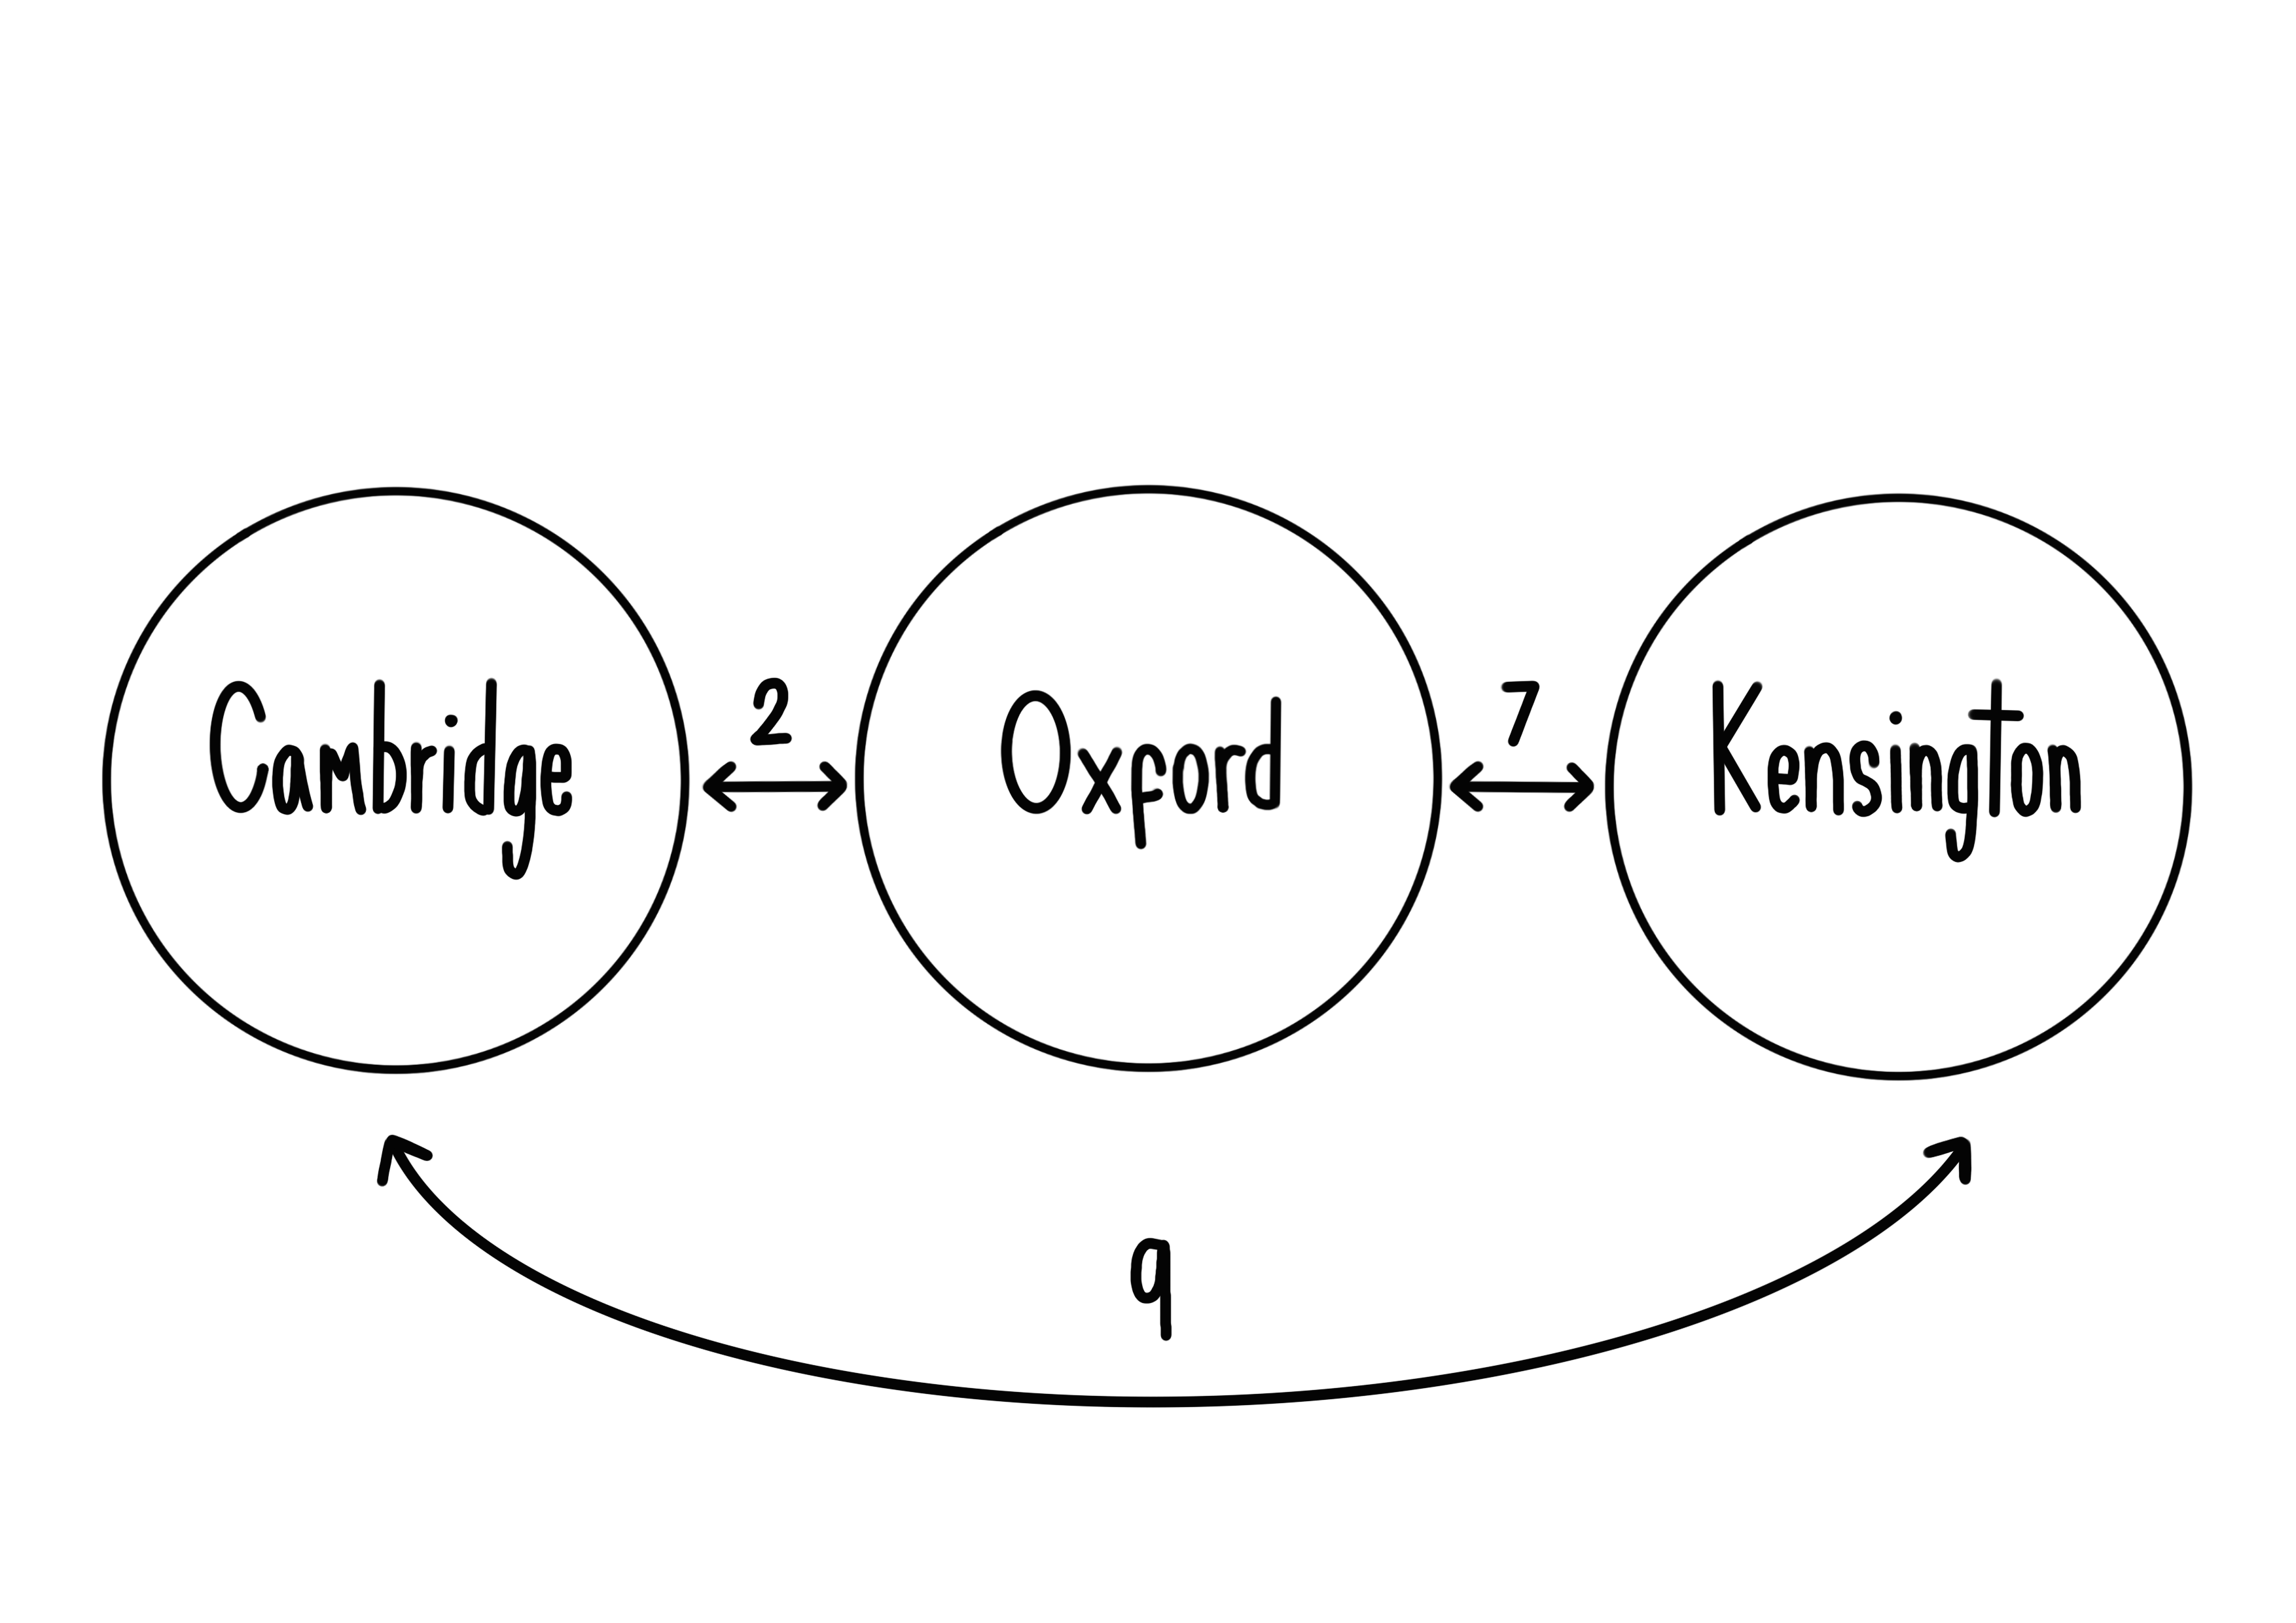
\includegraphics[width=0.5\textwidth]{trivialTSP.png}\\
\vspace{0.5cm}
A more complex instance:\\
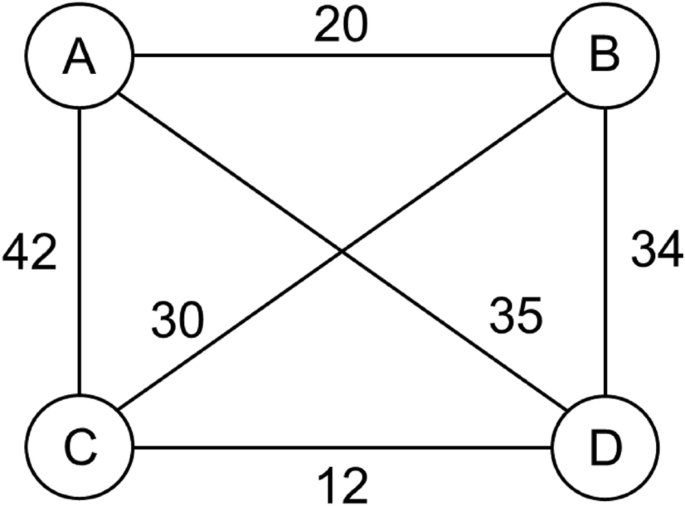
\includegraphics[width=0.5\textwidth]{HarderTSP.png}

\section{Big O-Notation}
Big-O notation describes how an algorithm's running time grows with input size. For input size $n$, an $O(n)$ algorithm scales linearly while $O(n^2)$ scales quadratically; polynomial-time algorithms ($O(n^k)$ for constant $k$) are considered tractable. Asymptotic notation abstracts machine-dependent constants and lower-order terms, enabling objective comparison of algorithmic efficiency.

\section{Sets and Set Notation}
A set is a well-defined collection of distinct objects. Useful symbols:
\begin{itemize}
    \item $\in$ — element of (e.g., $3\in\{1,2,3\}$)
    \item $\notin$ — not an element
    \item $\subseteq$ — subset
    \item $\cup,\ \cap$ — union, intersection
    \item $\setminus$ — set difference
\end{itemize}

\section{P}
The class $\mathbf{P}$ contains decision problems decidable by a deterministic Turing machine in polynomial time. Formally, $L\in\mathbf{P}$ if some deterministic Turing machine $M$ decides membership in $L$ in time $O(|x|^k)$ for some constant $k$.

\section{NP}
The class $\mathbf{NP}$ contains decision problems whose positive instances admit short certificates verifiable in polynomial time by a deterministic Turing machine. Formally, $L\in\mathbf{NP}$ if there exists a polynomial-time verifier $V(x,y)$ and polynomial $p$ such that $x\in L \iff \exists y, |y|\le p(|x|), V(x,y)=1$. Many natural combinatorial problems, including TSP, are NP-complete~\cite{karp1972,held1962}.

\section{Our Question}
The guiding problem is whether $\mathbf{P}=\mathbf{NP}$. We know $\mathbf{P}\subseteq\mathbf{NP}$, but equality remains open~\cite{arora2009}. This paper examines barriers that rule out broad classes of proof techniques rather than attempting a resolution.

\newpage
\chapter{Relativisation}
\subsection{Introduction to Relativisation}
One of the most important --- and possibly oldest --- barriers to resolving \textit{P vs NP} is known as \textit{relativisation}.
This idea was first formalised by three mathematicians in 1975, showing that a large group of mathematical proof methods face a fundamental limitation.
This limitation lies in their inability to separate the complexity classes discussed earlier when introducing \textit{Big O Notation}.
At its core, relativisation involves measuring how these complexity classes behave when given access to an \textit{"Oracle"}, and how an algorithm's reasoning encounters a limit when this additional power is introduced.

Relativisation refers to the property of certain proof techniques that remain valid when both complexity classes are given access to the same oracle. This concept is central to understanding why many classical approaches fail to resolve the P vs NP question. The following sections formalise the notion and discuss its implications for computational complexity.

\section{Oracles}
Defined by \cite{arora2009}:\\
Much like the legendary Oracle of Delphi, an \textit{Oracle} in complexity theory can provide an instant solution to a given subproblem.
It is an abstract tool—considered a 'black box' --- that never reveals how it reaches its answer, only that it does.
We refer to any \textit{Turing Machine} with access to such a tool as an \textit{Oracle Turing Machine}, which may query the oracle at any point during computation.
A relatable instance could be whilst driving you use a GPS, this tool does not show you how it gets its result however you will tend to trust it.
In that moment, using this information to guide your solution makes you behave almost like an \textit{Oracle Turing Machine}.
We denote this formally as $\mathbf{P^A}$ or $\mathbf{NP^A}$, meaning class $\mathbf{P}$ (or $\mathbf{NP}$) relative to oracle $A$.

\section{How does it apply to a resolution?}
A proof technique is said to \textit{relativize} if the logic of the proof still holds when both complexity classes are given access to the same oracle.
However, relativization as a method cannot resolve questions like $\mathbf{P = NP}$, as shown by Baker, Gill, and Solovay \cite{baker1975relativizations}.\\
They constructed two oracles, $A$ and $B$, such that:
\begin{itemize}
    \item $\mathbf{P^A = NP^A}$ (i.e., relative to oracle $A$, $\mathbf{P}$ and $\mathbf{NP}$ are equal)
    \item $\mathbf{P^B \neq NP^B}$ (i.e., relative to oracle $B$, they are distinct)
\end{itemize}
Any proof method that relativises will yield inconsistent results depending on the oracle. Consequently, such techniques cannot resolve \textit{P vs NP}, as they fail in certain relativised scenarios. This eliminates a large class of approaches; any successful proof must go beyond relativization.

\section{$\mathbf{P^A = NP^A}$}
The following are not real computational Oracles, entirely literary devices to simplify the idea for your consumption:
An example for this could be something as trivial as an oracle that simply returns the answer for our problem.
If our Salesperson is given a GPS (Oracle) with the ability to return the correct path, our problem becomes trivial and solvable in $\mathbf{P}$ relative to our Oracle.
A slightly less obvious case but more tedious could be a similar Oracle that simply alerts the Salesperson if they are going the wrong way.
This would make it so that our Salesperson never follows an incorrect path for more than 1 step.
Making their pathfinding efficient.

\section{$\mathbf{P^B \neq NP^B}$}
Let's imagine a new Oracle --- a weaker one.
Instead of being able to tell the Salesperson the best route, Oracle $B$ simply answers a limited amount of \textit{yes or no} questions.
The Salesperson may ask: "Is there a route shorter than 100 miles?" or "Is there a route that visits in alphabetical order?"
These answers, while marginally informative, do not reduce the core difficulty of constructing a full path, yet still offer a form of assistance with our planning.
In this case, the Salesperson still must explore a super-polynomial number of routes to construct a valid path, despite being able to verify a given solution efficiently.
In this case our Salesperson has no noticeable change in ability to verify the correctness of their path.
And the same is shown in their ability to plot the path.
Thus giving $\mathbf{P^B \neq NP^B}$.

\section{Reflection}
As \cite{aaronson2005philosophers} argues, relativization reflects a deeper philosophical boundary.
Just as some truths lie beyond formal proof, some complexity class separations may lie beyond the reach of techniques that relativize.
I see this as a crippling blow to many attempts at solving this problem.
This is because a method of proof could have no link whatsoever to these Oracles yet if the Oracle's application maintains the integrity of the proof then a barrier most would not consider has prevented the proof.
Whilst this barrier does prove devastating it does present a deeper beauty between philosophy and mathematics, that i must agree with Aaronson.

\newpage
\chapter{Natural Proofs}
\section{Introduction to Natural Proofs}
Simply put, a \textit{Natural Proof} is a method that works on many different functions and is easy to apply.  
A property $\mathcal{\pi}$ is said to be \textbf{natural} if:
\begin{itemize}
    \item \textbf{Constructivity}: Given the truth table of a Boolean function $f$, we can determine whether $f \in \mathcal{\pi}$ in polynomial time.
    \item \textbf{Largeness}: A non-negligible portion of all Boolean functions satisfy $\mathcal{\pi}$.
\end{itemize}

Natural proofs are a class of techniques in circuit complexity that are both efficiently checkable and broadly applicable. These methods have been instrumental in establishing lower bounds, but their limitations are profound when considering the separation of P and NP. The following section defines natural proofs formally and outlines their impact on complexity theory.

This concept can be illustrated by analogy\footnote{For example, an algorithm designed to detect AI-generated essays may be effective initially, but once its criteria are known, students can adapt their writing to evade detection. Similarly, if a detection method is too broad, it may incorrectly flag legitimate work.}. 
Constructivity refers to the property that a method can be efficiently applied, while largeness means it applies to a significant portion of cases.
This is best described by analogy.  
Imagine you're an English teacher --- a strict one --- who sets an essay for homework every lesson. You begin to suspect several students are using AI to write their essays.  
To catch them, you develop an algorithm that detects AI-generated writing.
Maybe it looks for excessive use of em-dashes or unnatural phrasing.
This algorithm is simple and can be applied to \textit{every} essay you mark.  
However, once students realise how it works, they adapt their writing style to evade detection.  
This captures the flaw with Constructivity: if your method is too effective and too public, it can be countered.
Largeness suffers a related issue. If your detection method works on too \textit{many} types of cheating --- copied essays, paraphrasing, ChatGPT, etc. --- then you're likely catching even legitimate work, or again being too general to be reliable.
\vspace{0.5cm}
\newline
We care whether a proof is \textit{natural} because many known lower-bound techniques are.  
This becomes especially relevant when we're trying to prove the \textit{lower bound} (minimum time to run) of a function $f$ --- that is, the fastest possible way to compute $f$.  
If we can do this, we may be able to show that $f \notin \mathbf{P}$.
\vspace{0.5cm}
\newline
On the surface, this seems like the perfect tool: if a problem looks hard and we can formally show it resists all efficient solutions, we've made progress toward proving it's not in $\mathbf{P}$.
But as we'll soon see, this tool cuts too deep --- and ends up breaking things we depend on, like cryptography.


\section{Circuit Complexity}
Before diving deeper into the limitations of Natural Proofs, we must take a step back and understand one of the main battlegrounds for proving $\mathbf{P \ne NP}$ --- \textbf{circuit complexity}.
Refer to our Salesperson.
Suppose instead of solving each map manually, they could build a dedicated machine for each map size --- a custom calculator of sorts made entirely of logic gates (AND, OR, NOT).
This machine would take a list of towns and output the shortest route.
In computational terms, this machine is a \textbf{Boolean circuit}.
Circuits don't run sequentially like an algorithm.
They are a set arrangement of gates that perform a binary operation.
Each value of $n$ gets a separate circuit.
We intend to keep these circuits small.
If we can prove that no small circuit can satisfy a problem, we have proven that the problem does not lie in $P$.
In doing so, proving $\mathbf{P \ne NP}$.
\vspace{0.2cm}
\textbf{Formally:}
The \textit{circuit complexity} $C(f)$ of a Boolean function $f : \{0,1\}^n \rightarrow \{0,1\}$ is the size of the smallest Boolean circuit that computes $f$ correctly on all inputs.
\vspace{0.1cm}
Referring back to our Salesperson, if the smallest circuit they can build for the TSP grows faster than any polynomial in $n$, this proves that we need \textit{super-polynomial} resources.
This would strongly suggest $\mathbf{P \ne NP}$.
\vspace{0.2cm}
Despite decades of mathematicians attempting to prove the lower bounds of problems in $\mathbf{NP}$, it has proven difficult.
Many of the proof techniques used are considered \textit{Natural}.
\begin{quote}
    "If we can prove that no small circuit solves a problem, we show that even the smartest shortcut-the most efficient mental 'machine' --- won't help our Salesperson beat the clock."\\
    - Inspired by~\cite{fortnow2009status}
\end{quote}

\section{Pseudorandom Functions}
Pseudorandom Functions (PRFs) are a core idea in cryptography.  
They are functions that look random, but are actually completely deterministic.  
To anyone without the secret key, the outputs seem unpredictable --- even though they're generated by a fixed rule.
This idea is essential for secure communication.  
If you can't tell the difference between a random number and one generated by a PRF, then you also can't reverse-engineer passwords, decode messages, or guess encryption keys.
Here's the link to Natural Proofs:  
If a proof method is both constructive and large, it may inadvertently undermine cryptographic assumptions by distinguishing pseudorandom functions, which is undesirable.\footnote{This is analogous to a security scanner that is so sensitive it detects legitimate or confidential items, illustrating the unintended consequences of overly broad detection methods.}

\section{Natural Proofs and Cryptography}
The discovery of natural proofs was initially seen as a breakthrough, providing a new angle from which to tackle the P vs NP question.
However, this hope was tempered by a sobering realisation: many natural proof techniques, while powerful, are also potentially dangerous.
They can be too revealing, exposing structural weaknesses in problems that are otherwise secure under cryptographic scrutiny.
The crux of the issue lies in the \textbf{largeness} requirement of natural proofs.
If a proof method is constructive and large, and still manages to prove a circuit lower bound for functions in $\mathbf{NP}$, it must also contradict the existence of pseudorandom functions.
This means that the search for new lower-bound techniques must avoid being \textit{natural} in this precise technical sense - a significant restriction.

\section{An Analogy}
Imagine you're running airport security.  
You build a fast, effective scanner that flags any suspicious-looking bag based on known patterns --- \textit{density, shape, wiring}.
It's fast enough to run on every passenger and catches most known threats.
This is your \textit{constructive} and \textit{large} method.
But what if attackers knew exactly how your scanner worked?  
They could design luggage that looks perfectly normal to your algorithm --- even if it's dangerous.
Now, imagine someone builds a new scanner that works so well it catches even these disguised threats.
You get excited: maybe this new system will finally make flying totally safe.
But then someone points out a terrifying implication:  
\textit{If this scanner works as described, it would also catch military stealth tech. Or diplomatic pouches. Or even encrypted test samples from trusted researchers.}
In short --- the scanner is \textit{too good}.  
If it works, it breaks things it wasn't meant to break.
That's the heart of the \cite{razborov1994} result.
If your method is constructive (efficient) and large (applies broadly), then it's strong enough to detect pseudorandom functions --- which modern cryptography says you shouldn't be able to do --- \cite{arora2009}.  
So unless we want to throw out the internet, these proof methods can't work.


\section{Consequences of a Natural Barrier}
The Razborov-Rudich insight does not just crumble our hope of a proof.
It fundamentally changes where we have to look for a proof for $\mathbf{P \ne NP}$.
Their proof showed us that any proof method that satisifies the criteria to be \textit{Natural} would allow us to distinguish between pseudorandom and random functions.
Something assured to be computationally impossible under standard cryptographic assumptions.
In short: if your proof techniques can work broadly and efficiently it is too broad to break the foundations of Cryptography.
So unless you are willing to fundamentally shatter the foundations of the modern internet your technique cannot be sufficient.\\
This creates a barrier with serious consequences:
\begin{itemize}
    \item It disqualifies many previously successful proof techniques, especially those that proved circuit lower bounds for simpler problems.
    \item It suggests that if $\mathbf{P \ne NP}$ is true, then any successful proof must avoid being natural - it must violate constructivity, largeness, or both.
    \item It highlights a surprising link between cryptography and complexity theory: breakthroughs in one domain may endanger assumptions in the other.
\end{itemize}
Return to our Salesperson:
Imagine you try to expose their inefficiency by building a test, a kind of security scanner for bad routes.
But every time you make it strong enough to work, it starts scanning and breaking real-world encrypted data.
In trying to catch the Salesperson, you have also accidentally hacked a bank.
The scanner is too powerful to be safely used.

\begin{quote}
    "Natural proofs aren't too weak to prove $\mathbf{P \ne NP}$ - they're too powerful.
    They solve more than they should, and in doing so, they violate assumptions we rely on elsewhere."\\
    - Adapted from \cite{razborov1994}
\end{quote}

While this result does not resolve the central question, it establishes that any proof of $\mathbf{P \ne NP}$ must avoid a large class of techniques.
\vspace{3cm}

\newpage
\chapter{Prerequesites to Algebrization}
This chapter briefly revisits Boolean circuits, oracles, and arithmetization, as these concepts underpin the algebrization barrier. For detailed definitions, see earlier chapters.

\section{Boolean Circuits}
Boolean circuits are networks of logic gates designed to solve computational problems for fixed input sizes. Their relevance to complexity theory and lower bounds is discussed in Chapter 2.

\section{Relativization and Oracles}
Relativization refers to proof techniques that remain valid when both complexity classes are given access to the same oracle. Oracles are abstract computational devices that provide instant solutions to subproblems. See Chapter 3 for formal definitions and implications.

\section{Arithmetization}
Arithmetization is the process of transforming Boolean functions into polynomials, enabling the use of algebraic techniques in complexity theory. Its significance for interactive proofs and the IP = PSPACE result is discussed in Chapter 4.

The result that $\mathbf{IP = PSPACE}$, established by Shamir~\citep{shamir1992ip}, demonstrated that interactive proof systems are as powerful as polynomial space algorithms. This equivalence revealed a deep connection between communication-based verification and computational resources, expanding the scope of problems that can be efficiently verified through interaction.

\newpage
\chapter{Algebrization}
\section{What is Algebrization?}
Previously we explored giving our Salesperson access to an \textit{Oracle} and saw how it allowed them to bypass certain computations.
We also saw how replacing rigid boolean with flexible logic we could achieve powerful results.
When we combine these we get \textit{algebrization}.
This was mentioned previously in our Prerequesite knowledge.

\begin{quote}
    "An algebrizing technique is one that works even when the algorithm can query both the function and its low-degree polynomial extension."\\
    - \cite{arora2008algebrization}
\end{quote}
A technique is formally said to \textit{algebrize} if it continues to work when both the Oracle $A$ and its low-degree extension $\tilde{A}$ are available.
These extensions come from viewing Boolean functions no longer as black boxes but polynomials.\\ 
Our Salesperson would previously ask the GPS if a shortcut existed.
Now they can know if a road is open and get an update on the terrain.
This makes no mystery to be revealed with the answer and mathmatical logic behind it.

\section{Why It Mattered}
Until now, our Salesperson had relied on his magic assistant (Oracle) or map (algebra).
Now imaghine the power of our Salesperson with both.
They would be able to conquer his problem trivially.
This intuition did seem strong.
One aspect of it revolutionised with a proof near our desired overarching problem.
And the other is an intrinsic property.
As \cite{arora2009} note, algebrization "combines the strengths of both relativization and arithmetization", it was a natural progression from our current techniques.
This is where the optimism runs dry unfortunately.

\section{The Barrier Itself}
\cite{arora2008algebration} introduced the concept formally and then dismantled it.
They showed that techniques that combine the strengths of Oracles and algebraic resoning are not strong enough to resolve $\mathbf{P}$ versus $\mathbf{NP}$.  
They constructed two oracles, $A$ and $B$, and their corresponding algebraic extensions $\tilde{A}$ and $\tilde{B}$, such that:
\begin{itemize}
    \item $\mathbf{P^A = NP^A}$ --- relative to Oracle $A$, the two classes collapse
    \item $\mathbf{P^B \ne NP^B}$ --- relative to Oracle $B$, the separation holds
\end{itemize}
When algorithms were allowed to query the low-degree polynomial extensions $\tilde{A}$ and $\tilde{B}$, the results differed.
This proved that any technique that works under algebraic Oracle access must fail to decide $\mathbf{P = NP}$.
\begin{quote}
    “The relativizing and arithmetizing barriers can be unified under the notion of algebrization --- and this unified barrier still fails to separate complexity classes like $\mathbf{P}$ and $\mathbf{NP}$.”\\
    - \cite{arora2008algebrization}
\end{quote}

Our Salesperson is now equipped with everything --- a GPS that answers instantly and a map of highest resolution.
Despite the armoury presented they still cannot prove the existence of an efficient way to visit all the towns.
The tools are as advanced as possible, but the truth remains obscured.
The significance of this result not only lay in its ability to reveal a new barrier but because it showed that even \textit{hybrid methods} were still not enough.
It unified previous barriers and then extended them, proving that even the most powerful techniques known may not be enough, even united.
For a brief moment, algebrization felt like the next great leap.
But it turned out to be the next great limitation.

\section{What algebrization Tells Us}
Our Salesperson has tried everything.
Simple algorithms.
Oracles for instantaneous answers.
Powerful mathematical maps have been used.
And even the final two in parallel.
Yet we are still no closer to proving if a solution exists.
Somewhere beyond the barriers of this report.
The road our Salesperson needs does exist, but it is hidden behind walls our current tools cannot penetrate.
This is not a failure for complexity theory.
It's a challenge, a challenge to be met by future computer scientist and mathematicians.
A new barrier does not close doors to discovery instead will leave an open window into the understanding of our world and maths itself.
This is not discouragement but a direction and foundation to guide the next generation.
\begin{quote}
    "Algebrization subsumes the known barriers of relativization and natural proofs, and yet it too falls short of separating $\mathbf{P}$ from $\mathbf{NP}$. We must look elsewhere."\\
    -\cite{arora2008algebrization}
\end{quote}

\section{What Does This Mean?}
It means that if $\mathbf{P \ne NP}$ --- and many believe it is --- the proof must lie somewhere we have not yet looked.
Somewhere beyond the barriers of this report.
The road our Salesman needs does exist, but it is hidden behind walls our current tools cannot penetrate.
This is not a failure for complexity theory.
It's a challenge, a challenge to be met by future computer scientist and mathematicians.
A new barrier does not close doors to discovery instead will leave an open window into the understanding of our world and maths itself.
This is not discouragement but a direction and foundation to guide the next generation.
\begin{quote}
    "Algebrization subsumes the known barriers of relativization and natural proofs, and yet it too falls short of separating $\mathbf{P}$ from $\mathbf{NP}$. We must look elsewhere."\\
    -\cite{arora2008algebrization}
\end{quote}

\newpage
\chapter{Conclusion}

\section{Summary of Barriers and Future Directions}
The investigation into the P vs NP problem has revealed three principal theoretical barriers: relativisation, natural proofs, and algeisation. Each barrier demonstrates that broad classes of proof techniques are fundamentally limited in their ability to resolve the question. Relativisation shows that techniques invariant under oracle access cannot distinguish P from NP. Natural proofs are ruled out by cryptographic assumptions, as they would compromise pseudorandomness. Algeisation unifies and extends these barriers, indicating that even hybrid approaches are insufficient.

These results suggest that future progress will require fundamentally new proof techniques that circumvent these limitations. Promising directions include non-relativising and non-natural methods, deeper exploration of circuit complexity, and connections to other areas such as algebraic geometry or quantum computation. Continued research into the structure of complexity classes and the development of novel mathematical tools remains essential.

The persistence of these barriers highlights the depth of the P vs NP problem and the need for innovative approaches. While the question remains unresolved, the identification of these obstacles has refined the search for a solution and clarified the boundaries of current knowledge.

\section{Lessons from Barriers}
These barriers should not be seen as failures but as \textit{refinements of knowledge}. Each negative result narrows the search space for future breakthroughs. For example, Razborov and Rudich's work forced a shift away from ``natural'' methods and toward approaches that violate constructivity or largeness. Similarly, algebrization redirected attention to techniques that move beyond both algebraic extensions and oracle relativisation.  

Recent research supports this perspective. Williams (2022), in \textit{Barriers Are Not Limits}, argues that while barriers rule out broad classes of techniques, they do not prohibit all possible methods. Instead, they should be seen as signposts: telling researchers where not to look, but also highlighting gaps where unconventional ideas might emerge. In this sense, the barriers are both restrictive and constructive---shaping the evolution of complexity theory itself.  

\section{Personal Reflection}
In undertaking this project, it became clear that explaining advanced results is not only about accuracy but also about accessibility. Initial drafts were overly technical and inaccessible; restructuring to include prerequisite sections and using analogies helped bridge this gap. However, it is now recognised that metaphor was sometimes over-relied upon at the expense of concision. A more balanced approach would have improved the clarity and academic tone.  

The difficulty of engaging with algebrisation, where accessible treatments were scarce, was underestimated. Relying heavily on Arora and Barak provided a solid foundation but limited breadth. If repeating this project, integrating more recent work on proof complexity and derandomisation would be prioritised, and a stricter referencing style would be adopted from the outset to avoid inconsistencies.  

Despite these limitations, the project developed skills in \LaTeX, structured research management (via Git and logs), and critical reading of advanced literature. More importantly, it provided a deeper appreciation of how ``negative'' results in mathematics can still be progress: barriers are not endpoints but guideposts.  

\section{Why the Road Remains Untraveled}
The heart of my project was the question "What are the main theoretical barriers to resolving P vs NP?"
Our goal to understand how it resisted solution for over 50 years by some of history's greatest minds.
Through the lens of a travelling salesperson—modelled on the $NP$-complete Travelling Salesperson Problem (TSP)—the principal strategies developed in computer science were examined.
This metaphor illustrates the limitations of current approaches.
Beginning with \textbf{relativisation}, followed by \textbf{natural proofs} and their successor \textbf{algebrisation}.
The analysis demonstrates that existing techniques are insufficient.
These barriers function not only as technical limitations, but also as statements about the boundaries of mathematical knowledge and the principles required for rigorous proof.
For the hypothetical salesperson, these barriers manifest as both physical and technological constraints.
This exemplifies the nature of theoretical computer science and mathematics.
Each negative result refines collective understanding, and each limitation marks progress.
Expanding knowledge of ineffective approaches increases the likelihood of identifying successful ones.
\begin{quote}
    "Barriers are not endpoints --- they are waypoints. They tell us how far we've come, and where new paths must begin."\\
    -Inspired by themes in~\cite{arora2009}
\end{quote}
The question of $\mathbf{P}$ versus $\mathbf{NP}$ remains one of the deepest in both Maths and Computer Science.
And because of the work of those who identified these barriers we know something equally important.
\textbf{We know which paths to not follow and hopefully this can lead us to the correct path.}

\section{Personal Opinion}
Although the question of whether $P = NP$ remains unsolved, I personally believe that $P \ne NP$.
This conviction not only stems from the decades of failed proofs otherwise, but from a structural asymmetry between verification and construction.
It seems unlikely that all problems can be verified as efficiently as solved.
During the research for this project i encountered a paper called Differentiation of sets --- The general case~\cite{WeilDifferentiate}.
This paper allowed me to view through a more abstract lens --- such as the concept of calculus on sets I explored --- differences in how sets "change" under transformations or abstractions.
For those Mathematically-minded this is not dissimilar from taking the derivative.
In doing this the results appear to suggest a fundamental difference in character between $P$ and $NP$.
This difference then suggests they cannot be the same.
While this is not a formalised or even rigorous proof, it provides conceptual bases for understanding why such a collapse in complexity classes seems implausible.

\chapter*{Project Foundations}
\section*{Planning and Structure}
Orignally scoped to explain the P vs NP problem to a non-mathematical audience by exploring the three core barriers.
I underestimated the difficulty of sourcing accessibility material for algebrization.
In order to adjust for this i allocated myself additional time to read Arora and Barak's treatment \cite{arora2008algebrization}.
Then restructuring my draft to accomodate a dedicated prerequisite section.
The use of LaTeX --- A software used within mathematics to write papers --- added complexity to the formatting phase, but also taught me new skills in document management and academic writing.
I maintained a research log and planned section goals week by week, even using Git --- an application commonly used in coding and other endeavors to allow you to save and access from anywhere --- to allow a strong version control.
The final version being read now differs from my initial outline, but reflects clear evolution of myself and the project.
Progress was tracked using a weekly Gantt chart alongside an annotated research log.
These allowed me to record changes and give priority to certain topics.
This allowed me to identify metaphorical clarity's demand for precedence over technical depth, ensuring the final document was aligned to examiner criteria.

\section*{Literature Review}
This project draws upon a range of literature --- entirely academic --- in regards to complexity theory and foundational mathematics behind it.
The primary source used as the textbook by Arora and Barak, \cite{arora2009}, offering rigorous definitions and strong explanations in technical detail of everything mentioned in this report.
This is supported by the Razborov-Rudich paper, \cite{razborov1994}, formalising the concept of Natural Proof.
Fortnow's paper, \cite{fortnow2009status}, was mandatory for my understanding of circuit complexity and the progression of techniques used.
reflective work by \cite{aaronson2005philosophers} granted insight into the philosophical understanding of each barrier's result.
These sources were selected due to their academic credibility, relevance and clarity.
Where possible original papers were prioritised to ensure maximal accuracy ---  with secondary resources used to strengthen personal understanding to put such knowledge into this paper.
Whilst some sources were seminal and authoritative, several alternatives were considered.
Sipser's textbook was initially reviewed for its coverage of relativization, but was deemed too introductory for my project's goals.
Similarly, more recent survey papers were considered, few offering deeper insights than Arora and Barak or Razborov-Rudich.
The sources chosen therefore reflect not just authority but suitability for explanation and metaphor.
Future versions of this work could benefit from incorporating more recent developments and derandomization literature.

During the research phase of the project, I encountered newer papers such as "Barriers Are Not Limits"~\citep{williams2022barriers}, which provided reflective commentary on the state of complexity theory.  
Additional sources, including Aaronson's blog, *Shtetl-Optimized* (Aaronson, 2005–2024)\footnote{See Scott Aaronson's blog, \textit{Shtetl-Optimized}: \url{https://www.scottaaronson.com/blog/}.}, were consulted for informal perspectives and clarification of technical concepts.  
While the blog is academically rigorous, its depth and informality were not always suited to the scope of this project.

\section*{Skills and Personal Development}
This project's completion had taught me more than theoretical complexity.
Beginning with a surface-level understanding of P vs NP, developing the ability to explain cutting-edge research.
Translating complex topics via analogy --- particularly with TSP --- deepened my respect in both communication and mathematics.
Especially during my work on algebrisation with scarce introductory treatments.
These skills have become valuable to my arsenal of problem solving methods.

\bibliographystyle{agsm}
\bibliography{references}

\newpage
\chapter*{Glossary}
\begin{description}
    \item[Complexity Class] A set of decision problems grouped by the resources (such as time or space) required to solve them using a computational model.
    \item[P] The class of decision problems solvable by a deterministic Turing machine in polynomial time.
    \item[NP] The class of decision problems for which a solution can be verified in polynomial time by a deterministic Turing machine.
    \item[TSP (Travelling Salesperson Problem)] An NP-complete problem that asks for the shortest possible route visiting each city exactly once and returning to the origin city.
    \item[Oracle] An abstract computational device that can instantly solve a specific subproblem, used to study the limits of proof techniques.
    \item[Relativization] A property of proof techniques that remain valid when both complexity classes are given access to the same oracle.
    \item[Natural Proof] A type of proof technique characterised by constructivity and largeness, shown to be insufficient for separating P from NP under standard cryptographic assumptions.
    \item[Algebrization] A proof technique that combines access to both an oracle and its algebraic extension, shown to be insufficient for resolving P vs NP.
    \item[Boolean Circuit] A network of logic gates designed to solve a specific computational problem for a fixed input size.
    \item[Pseudorandom Function] A deterministic function that appears random to any efficient algorithm lacking the secret key, fundamental in cryptography.
    \item[Verifier] An algorithm that checks the validity of a proposed solution (certificate) for a decision problem.
    \item[Polynomial Time] Computation whose running time is bounded by a polynomial function of the input size.
    \item[Lower Bound] A proven minimum on the resources required to solve a problem, such as time or circuit size.
\end{description}

\end{document}